\documentclass{beamer}
\usetheme{Berkeley}
\usecolortheme{default}
\setbeamertemplate{items}[triangle]
\setbeamertemplate{sections/subsections in toc}[square]
\addtobeamertemplate{navigation symbols}{}{%
    \usebeamerfont{footline}%
    \usebeamercolor[fg]{footline}%
    \hspace{1em}%
    \insertframenumber/\inserttotalframenumber
}

\usepackage[T1]{fontenc}
\usepackage[utf8]{inputenc}

% Math
\usepackage{amsmath}
\usepackage{amsfonts}
\usepackage{amssymb}
\usepackage{amsthm}

% Algorithm & code listing
\usepackage{algorithm}
\usepackage[noend]{algpseudocode}
\makeatletter
\algrenewcommand\ALG@beginalgorithmic{\footnotesize}
\def\NoNumber#1{{\def\alglinenumber##1{}\State #1}\addtocounter{ALG@line}{-1}}

% Figures
\usepackage{subfloat}
\usepackage{caption}
\usepackage{subcaption}

\usepackage{biblatex}
\addbibresource{final.bib}

%Information to be included in the title page:
\title{Bayesian parameter synthesis for Markov population models.}
\author{Phung Nhat-Huy}
\date{\today}
\institute{University of Konstanz}
\titlegraphic{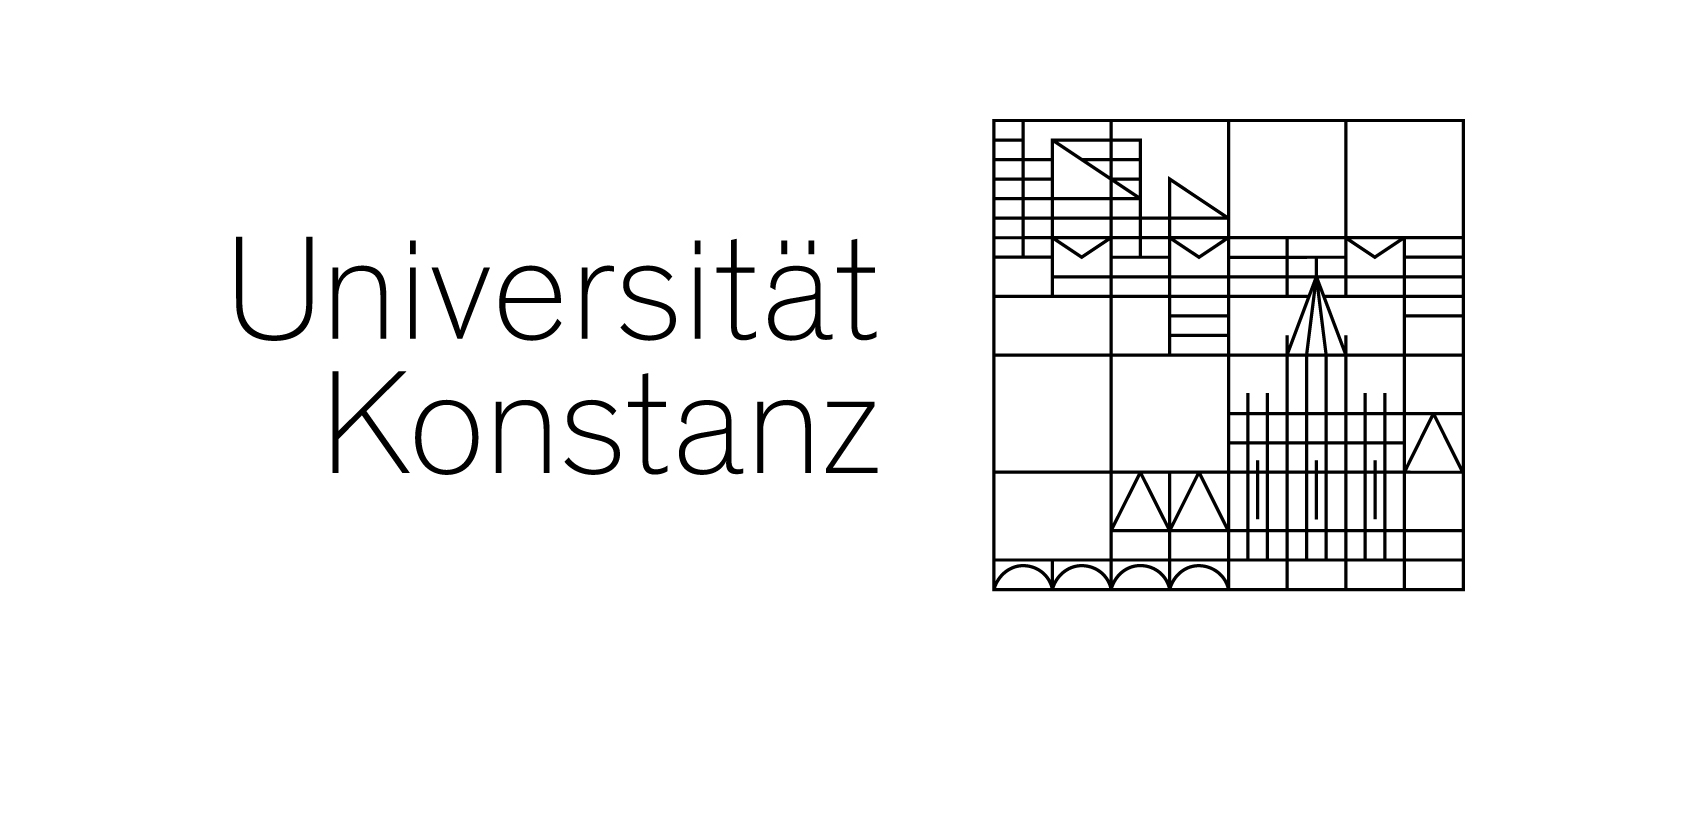
\includegraphics[width=5cm]{figures/unisignet-klein.jpg}}


\begin{document}

\frame{\titlepage}
\frame{\tableofcontents}

%%%%%%%%%%%%%%%%%%%%%%%%%%%%%%%%%%%%%%%%%%%%%%%%%%%%%%%%%%%%%%%%%%%%%%%%%%%%%%%%%%%%%%%%%%%%%%%%%%%%
\section{Motivation}
\begin{frame}
    \begin{center}
        \Huge Motivation.
    \end{center}
\end{frame}

\begin{frame}
    \frametitle{Motivation}
    \begin{itemize}
        \item We study the population dynamics of a system of interest. For example:
              \begin{itemize}
                  \item Number of online nodes in a computer network.
                  \item Number of surviving individuals in an epidemic model.
              \end{itemize}
        \item We study the population in a grey-box setup
              \begin{itemize}
                  \item Estimating the model's unknown attributes with experiment data of the
                        population at its steady state.
              \end{itemize}
    \end{itemize}
\end{frame}

\begin{frame}
    \frametitle{Motivation}
    \begin{itemize}
        \item Modeling population using a stochastic process (Markov population model
              \cite{kingman1969markov})
              \begin{itemize}
                  \item Discrete-time Markov chain
              \end{itemize}
        \item Parameterization: encoding the unknown attributes of a system by model parameters
              \begin{itemize}
                  \item Parametric discrete-time Markov chain \cite{katoen2016probabilistic}).
              \end{itemize}
    \end{itemize}
\end{frame}

\begin{frame}
    \frametitle{Motivation}
    As parameters represent unknown features of the system, it gives the following research
    questions
    \begin{itemize}
        \item \textit{(Parameter inference):} Given a set of data collected by observing the system,
              what can we know about its parameters?
        \item \textit{(Parameter synthesis):} Which values of parameters instantiate a model that
              satisfies a specific property of interest?
    \end{itemize}
\end{frame}

%%%%%%%%%%%%%%%%%%%%%%%%%%%%%%%%%%%%%%%%%%%%%%%%%%%%%%%%%%%%%%%%%%%%%%%%%%%%%%%%%%%%%%%%%%%%%%%%%%%%
\section{Preliminaries}
\begin{frame}
    \begin{center}
        \Huge Probabilistic model checking
    \end{center}
\end{frame}

\begin{frame}
    \frametitle{Discrete-time Markov chain}
    \footnotesize {
        \begin{definition}[Discrete Time Markov Chain \cite{baier2008principles}]
            \rm
            A \textit{Discrete-time Markov chain} (or DTMC in short) $\mathcal{M}$ is a tuple
            $(S,\mathbf{P}, \iota_{init}, AP, L)$, in which
            \begin{itemize}
                \item $S$ is a countable, non-emty set of \textit{states}
                \item $\mathbf{P}:S\times S \rightarrow [0,1]$ is the \textit{transition probability}
                      function such that
                      \begin{align*}
                          \forall s \in S : \sum_{s'\in S}\mathbf{P}(s, s') = 1
                      \end{align*}
                \item $\iota_{init}: S \rightarrow [0,1]$ is the \textit{initial distribution} such that
                      \begin{align*}
                          \sum_{s\in S} \iota_{init}(s) = 1
                      \end{align*}
                \item $AP$ is a set of \textit{atomic propositions}.
                \item $L: S \rightarrow 2^{AP}$ is the labelling function on states.
            \end{itemize}
        \end{definition}
    }
\end{frame}

\begin{frame}
    \frametitle{Bottom Strongly Connected Components}
    \footnotesize{
        \begin{definition}[Strongly Connected Component]
            \rm
            Let $\mathcal{M}=(S,\mathbf{P}, \iota_{init}, AP,L)$ be a DTMC. A subset $S'\subset S$ is
            \textit{strongly connected} if and only if for every pair $s_1,s_2\in S'$ there is a path
            between $s_1$ and $s_2$ which consists of only states in $S'$. If $S'$ has no superset
            $S''\subseteq S$, such that $S''$ is strongly connected, then $S'$ is a \textit{Strongly
                Connected Component}, or \textit{SCC} in short.
        \end{definition}

        \begin{definition}[Bottom Strongly Connected Component]
            \rm
            Let $\mathcal{M}=(S,\mathbf{P}, \iota_{init}, AP,L)$ be a DTMC and $S'\in S$ a Strongly
            Connected Component. $S'$ is also a \textit{Bottom Strongly Connected Component} (or
            \textit{BSCC} in short), if and only if there exist no state $s \in S\backslash S'$ that is reachable
            from any state in $S'$. If $|S'|=1$ then $S'$ is a \textit{trivial BSCC}. We denote
            $BSCC(\mathcal{M})\in S$ is the set of all BSCCs of $\mathcal{M}$.
        \end{definition}
    }
\end{frame}

\begin{frame}
    \frametitle{Example of DTMC}
    Algorithm by Knuth and Yao \cite{knuth1976complexity} to model a fair dice by a fair coin.
    \begin{figure}[H]
        \centering
        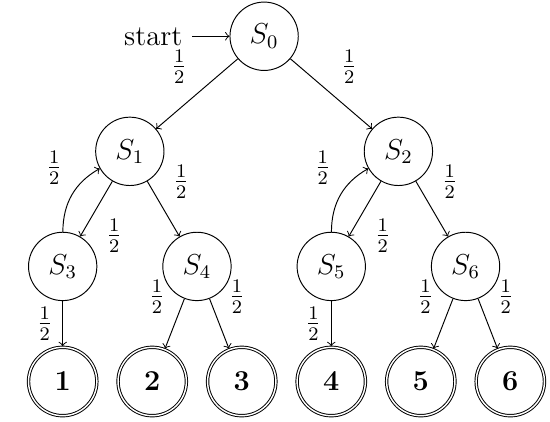
\includegraphics[width=0.4\textwidth]{figures/knuth_die_dtmc.png}
        \caption{DTMC model of Knuth-Yao die. There are six BSCCs labbeled "1" to "6"}
        \label{fig:knuth-die-dtmc}
    \end{figure}
\end{frame}

\begin{frame}
    \frametitle{Probabilistic Computational Tree Logic}
    \footnotesize{
        \begin{definition}[PCTL \cite{baier2008principles}]
            \rm
            The syntax of PCTL consists of state formulas and path formulas.
            \begin{itemize}
                \item State formulas are defined over $AP$
                      \begin{align*}
                          \Phi & ::= \text{true} \;|\; a \;|\; \Phi \;|\; \Phi_1 \wedge \Phi_2 \;|\; \Phi_1 \vee \Phi_2 \;|\;  P_{J}(\phi)
                      \end{align*}
                      where $a\in AP$, $\phi$ is a path formula, and $J\subseteq[0,1]$ is an interval.
                \item Path formulas
                      \begin{align*}
                          \phi & ::= \bigcirc \Phi \;|\; \Phi_1 \mathsf{U} \Phi_2 \;|\; \Phi_1 \mathsf{U}^{\leq n} \Phi_2
                      \end{align*}
                      where $\Phi,\Phi_1,\Phi_2$ are state formulas, and $n\in \mathbb{N}$.
            \end{itemize}
        \end{definition}
    }
\end{frame}

\begin{frame}
    \frametitle{Example of DTMC}
    Algorithm by Knuth and Yao \cite{knuth1976complexity} to model a fair dice by a fair coin.
    \begin{figure}[H]
        \centering
        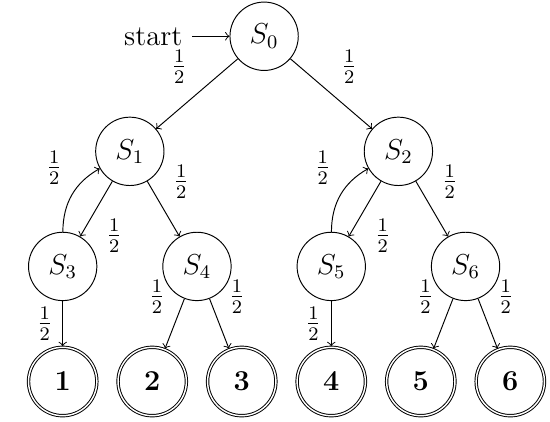
\includegraphics[width=0.4\textwidth]{figures/knuth_die_dtmc.png}
        \caption{DTMC model of Knuth-Yao die. There are six BSCCs labbeled "1" to "6"}
    \end{figure}
    The probability that the simulation eventually ends with the outcome "one dot" is equal to
    $\frac{1}{6}$:
    \begin{align*}
        P_{=\frac{1}{6}}(\texttt{True} \mathsf{U} \texttt{"1"})
    \end{align*}
\end{frame}


\begin{frame}
    \frametitle{Parametric discrete-time Markov chain}
    \footnotesize{
        \begin{definition}[Parametric discrete-time Markov chain \cite{junges2019parameter}]
            \rm
            A \textit{parametric discrete-time Markov chain} $\mathcal{M}_\theta$ is a tuple $(S, \theta,
                \mathbf{P}, \iota_{init}, AP, L)$ where
            \begin{itemize}
                \item $S$ is a countable, non-emty set of \textit{states}
                \item $\theta \in \mathbb{R}^n, n \in \mathbb{N}$ as the set of  parameters.
                \item $\mathbf{P}:S\times S \rightarrow \mathbb{Q}(\mathbf{x})$ is the \textit{transition
                          probability} function such that
                      \begin{align*}
                          \forall s \in S : \sum_{s'\in S}\mathbf{P}(s, s') = 1
                      \end{align*}
                \item $\iota_{init}: S \rightarrow [0,1]$ is the \textit{initial distribution} such that
                      \begin{align*}
                          \sum_{s\in S}\iota_{init}(s) = 1
                      \end{align*}
                \item $AP$ is a set of \textit{atomic propositions}
                \item $L: S \rightarrow 2^{AP}$ is the labelling function on states.
            \end{itemize}
        \end{definition}
    }
\end{frame}

\begin{frame}
    \frametitle{Example of DTMC}
    Algorithm by Knuth and Yao \cite{knuth1976complexity} to model a possibly unfair dice by two
    possibly unfair coins.
    \begin{figure}[H]
        \centering
        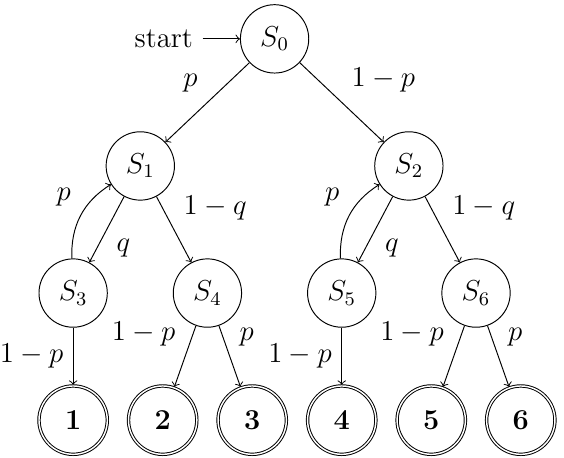
\includegraphics[width=0.4\textwidth]{figures/knuth_die_pdtmc.png}
        \caption{DTMC model of Knuth-Yao die with two possibly unfair coins. There are six BSCCs labbeled "1" to "6"}
        \label{fig:knuth-die-pdtmc}
    \end{figure}
\end{frame}

\begin{frame}
    \frametitle{Parameter synthesis}
    \begin{definition}[Parameter synthesis (Katoen \cite{katoen2016probabilistic})]
        Given a finite-state parametric Markov model, find the parameter values for which a given
        reachability property exceeds (or is below) a given threshold $\beta$.
    \end{definition}
\end{frame}

\begin{frame}
    \frametitle{Parameter synthesis}
    Katoen \cite{katoen2013model} summarizes the following methods on parameter synthesis of parametric DTMC:
    \begin{enumerate}
        \item \textit{Computing symbolic reachability probabilities (Daws \cite{daws2004symbolic},
                  Hahn \cite{hahn2011probabilistic})}: symbolic solving system of linear equations.
        \item \textit{Candidate region generation and checking (Kwiatkowska
                  \cite{kwiatkowska2006symmetry})}: partition the parameter space into \textit{safe} and
              \textit{unsafe} regions.
        \item \textit{Parameter lifting (\cite{quatmann2016parameter})} replace parametric
              transition system by a non-parametric one with transition labels are bounds from given
              intervals.
    \end{enumerate}
\end{frame}

\begin{frame}
    \frametitle{Example of DTMC}
    Given DTMC model $\mathcal{M}_{(p,q)}$ as in \ref{fig:knuth-die-pdtmc} and a property
    \begin{align*}
        \Phi = P_{\geq 0.2} (\texttt{True} \mathsf{U} \texttt{"1"})
    \end{align*}
    A Monte Carlo sampling using $p,q \sim Uniform(0,1)$ gives the following satisfying parameter values
    \begin{figure}[H]
        \centering
        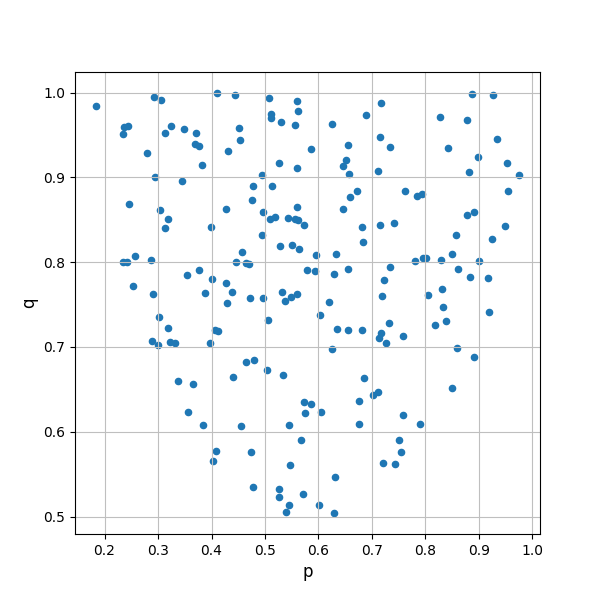
\includegraphics[width=0.4\textwidth]{figures/knuth_die_trueparams.png}
        \caption{Samples of $(p,q)$ that instantiate $\mathcal{M}_{(p,q)} \models \Phi$.}
        \label{fig:knuth-die-pdtmc-mc}
    \end{figure}
\end{frame}

%% Bayesian inference: 10 frames
\begin{frame}
    \begin{center}
        \Huge Bayesian inference
    \end{center}
\end{frame}

\begin{frame}
    \frametitle{Bayes theorem}
    \begin{definition}[Bayes theorem]
        \rm
        \begin{align*}
            \pi(\theta | D_{obs}) = \frac{P(D_{obs}|\theta)\pi(\theta)}{\int_\theta P(D_{obs}|\theta)\pi(\theta)d\theta}
        \end{align*}
        where
        \begin{itemize}
            \item $\pi(\theta)$ is the \textit{prior distribution}.
            \item $P(D_{obs}|\theta)$ is the \textit{likelihood}.
            \item $\int_\theta P(D_{obs}|\theta)\pi(\theta)d\theta$ is the \textit{marginal distribution}.
            \item $\pi(\theta | D_{obs})$ is the \textit{posterior distribution}
        \end{itemize}
    \end{definition}
\end{frame}

\begin{frame}
    \frametitle{Bayesian parameter estimation}
    \begin{itemize}
        \item With posterior distribution $\pi(\theta|D_{obs})$ we estimate the parameter $\hat{\theta}$ using Bayesian
              posterior mean.
              \begin{align*}
                  \hat{\theta} = \mathbf{E}[\theta] = \int_\theta \theta \pi(\theta|D_{obs}) d\theta
              \end{align*}
        \item In case we have samples from posterior distribution, for example a set of $N$ parameter values
              $(\theta_1,\ldots,\theta_N)$ sampled from the posterior distribution $\pi(\theta|D_{obs})$, the
              discrete form of posterior mean is used:
              \begin{align*}
                  \hat{\theta} \approx \mathbf{E}[\theta] \approx \sum_\theta \theta \pi(\theta|D_{obs})
              \end{align*}
    \end{itemize}
\end{frame}

\begin{frame}
    \frametitle{Approximation of  posterior distribution}
    \begin{itemize}
        \item Usually posterior distribution $\pi(\theta|D_{obs})$ has no analytical to evaluate
        \item We use sampling algorithms to draw samples from posterior distribution
              \begin{itemize}
                  \item Metropolis-Hastings
                  \item Sequential Monte-Carlo
                  \item Approximate Bayesian computation
              \end{itemize}
    \end{itemize}
\end{frame}

\begin{frame}
    \frametitle{Metropolis-Hastings}
    \footnotesize{
        \begin{algorithm}[H]
            \caption{Metropolis-Hastings Algorithm}
            \label{alg:mh}
            \begin{algorithmic}[1]
                \Procedure{Metropolis-Hastings}{}
                \State Init empty trace
                \State Init $\theta_{1}$ from $\pi(\theta)$
                \While{$i \leq N_{MH}$}
                \State Draw $\theta_{cand}$ from $Q(\theta'|\theta_{i-1})$
                \State Compute $\xi = \min(0, \ln(P(D_{obs}|\theta_{cand})) - \ln(P(D_{obs}|\theta_{i-1})))$
                \If{$\xi > 0 $}
                \State Accept $\theta_{cand}$, append to trace.
                \Else
                \State Draw a random number $u$ from $Uniform(0,1)$
                \If{$u \leq \exp(\xi)$}
                \State Accept $\theta_{cand}$, append to trace.
                \EndIf
                \EndIf
                \EndWhile
                \State Return $(\theta_1,\ldots,\theta_{N})$, $(w_1,\ldots,w_{N})$
                \EndProcedure
            \end{algorithmic}
        \end{algorithm}
    }
\end{frame}

\begin{frame}
    \frametitle{Metropolis-Hastings}
    Advantages of Metropolis-Hastings are:
    \begin{itemize}
        \item[+] Parameter transition only needs the computation of the likelihood function.
        \item[+] Computationally efficient, as marginal distribution is canceled out, and likelihood can
              be replaced by log-likelihood.
        \item[+] Simple to implement.
    \end{itemize}
    Disadvantages of Metropolis-Hastings are
    \begin{enumerate}
        \item[-] Highly probable to be stuck in a local maximum or minimum.
        \item[-] Not parallelizable
    \end{enumerate}
\end{frame}

\begin{frame}
    \frametitle{Sequential Monte-Carlo}
    \footnotesize{
        \begin{algorithm}[H]
            \caption{Sequential Monte Carlo Algorithm}
            \label{alg:smc}
            \begin{algorithmic}[1]
                \Procedure{Sequential-Monte Carlo}{}
                \State Draw $(\theta_1,\ldots,\theta_N)$ from $\pi(\theta)$ \algorithmiccomment {SMC initialization}
                \State $t \leftarrow 1$
                \While{$t \leq M$}
                \State Normalize $(w^{t-1}_1,\ldots,w^{t-1}_N)$  \algorithmiccomment{SMC correction step}
                \State Sample with replacement $(\theta^t_1,\ldots,\theta^t_N)$ \algorithmiccomment{SMC selection step}
                \NoNumber{\hspace{.5cm}} from $(\theta^{t-1}_1,\ldots,\theta^{t-1}_N)$ with probabilities $(w^{t-1}_1,\ldots,w^{t-1}_N)$
                \State $i \leftarrow 1$
                \While{$i \leq N$} \algorithmiccomment {SMC perturbation step}
                \State Draw $\hat{\theta}^t_i$ from $F_t(\theta^t | \theta^{t-1}_1,\ldots,\theta^{t-1}_N), 1\leq t \leq M$
                \State Mutate $(\theta^*_1,\ldots,\theta^*_{N_{MH}}), (w^*_1,\ldots,w^*_{N_{MH}}) \leftarrow MH(\hat{\theta}^t_i)$
                \State $\theta_i \leftarrow \theta^*_{N_{MH}}$
                \State $w_i \leftarrow w^*_{N_{MH}}$
                \EndWhile
                \EndWhile
                \State Return $(\theta_1,\ldots,\theta_{N})$, $(w_1,\ldots,w_{N})$
                \EndProcedure
            \end{algorithmic}
        \end{algorithm}
    }
\end{frame}

\begin{frame}
    \frametitle{Sequential Monte-Carlo}
    Sequential Monte Carlo algorithm has several advantages compared to Metropolis-Hastings
    algorithm.
    \begin{itemize}
        \item[+] Approximate multimodal distributions: $N$ particles moving independently.
        \item[+] Parallelizable.
    \end{itemize}
    However, Sequential Monte Carlo also has disadvantages:
    \begin{itemize}
        \item[-] Selection of perturbation and transition kernel is not trivial (Filippi
              \cite{filippi2013optimality}, and Silk \cite{silk2012optimizing}).
        \item[-] More difficult to implement.
    \end{itemize}
\end{frame}

\begin{frame}
    \frametitle{Approximate Bayesian Computation}
    A likelihood-free method
    \begin{itemize}
        \item used when likelihood has no analytical form, or the analytical form is
              expensive to be evaluated.
        \item estimates the likelihood $P(D_{obs}|\theta)$, or replace it by other
              measures.
    \end{itemize}
\end{frame}

\begin{frame}
    \frametitle{Approximate Bayesian Computation}
    \footnotesize{
        \begin{algorithm}[H]
            \caption{Approximate Bayesian Computation}
            \label{alg:abc-reject}
            \begin{algorithmic}[1]
                \Procedure{Approximate-Bayesian-Computation}{}
                \State Select a proposal distribution $\pi(\theta)$
                \State $i \leftarrow 1$
                \While{$i \leq N$}
                \State Draw a random particle $\theta$ from $\pi(\theta)$
                \State Simulate data $D_{sim}$ from $\mathcal{M}_\theta$
                \If{$d = \delta(D_{sim}, D_{obs}) < \epsilon$}
                \State $\theta_i \leftarrow \theta$
                \State $w_i = d$
                \EndIf
                \EndWhile
                \State Return $(\theta_1,\ldots,\theta_N)$, $(w_1,\ldots,w_N)$
                \EndProcedure
            \end{algorithmic}
        \end{algorithm}
    }
\end{frame}

\begin{frame}
    \frametitle{Approximate Bayesian Computation}
    Advantages of Approximate Bayesian Computation are:
    \begin{itemize}
        \item[+] Likelihood-free: applicable when the likelihood has no analytical form or there is no
              likelihood.
        \item[+] Easy to implement.
    \end{itemize}
    However, Approximate Bayesian Computation has drawbacks:
    \begin{itemize}
        \item[-] How to select a distance threshold $\epsilon$ so that the posterior is closely
              approximated? \cite{sisson2007sequential}
        \item[-] How to choose a summary statistic to capture sufficient information?
              \cite{csillery2010approximate}
    \end{itemize}
\end{frame}

\begin{frame}
    \frametitle{Parameter synthesis and Parameter inference}
    What are the differences between parameter inference and parameter synthesis?
    \begin{table}[]
        \begin{tabular}{|l|l|l|}
            \hline
                                       & Input                      & Ouput                      \\ \hline
            \begin{tabular}[c]{@{}l@{}}Parameter\\ inference\end{tabular} & \begin{tabular}[c]{@{}l@{}}Model $\mathcal{M}_\theta$\\ Observed data $D_{obs}$ \end{tabular} & \begin{tabular}[c]{@{}l@{}}Parameter estimation\\ $\hat{\theta}$\end{tabular} \\ \hline
            \begin{tabular}[c]{@{}l@{}}Parameter\\ synthesis\end{tabular} & \begin{tabular}[c]{@{}l@{}}Model $\mathcal{M}_\theta$\\ Reachability property $\Phi$ \end{tabular} & \begin{tabular}[c]{@{}l@{}}$(\theta_1,\ldots,\theta_N)$ \\ $\forall \theta_i \in (\theta_1,\ldots,\theta_N):$ \\$\mathcal{M}_{\theta_i}\models\Phi$\end{tabular} \\ \hline
        \end{tabular}
    \end{table}
\end{frame}


%%%%%%%%%%%%%%%%%%%%%%%%%%%%%%%%%%%%%%%%%%%%%%%%%%%%%%%%%%%%%%%%%%%%%%%%%%%%%%%%%%%%%%%%%%%%%%%%%%%%
\section{Contributions}
\begin{frame}
    \begin{center}
        \Huge Contributions
    \end{center}
\end{frame}

\begin{frame}
    \frametitle{Framework design}
    \begin{itemize}
        \item In this thesis, we combine parameter synthesis and parameter inference into a
              data-informed parameter synthesis framework.
              \begin{itemize}
                  \item Sample a set of parameter values which satisfy a property of interest
                        \textit{(parameter synthesis)} and use it to estimate a parameter value which
                        the observed data is likely to be simulate from \textit{(parameter inference)}.
              \end{itemize}
    \end{itemize}
\end{frame}

\begin{frame}
    \frametitle{Framework design}
    \begin{itemize}
        \item Given experiment data of a system at its steady state and a property of interest
              \begin{itemize}
                  \item \textit{Bayesian parameter inference:} apply different sampling algorithm to
                        approximate the posterior distribution of parameter.
                  \item \textit{Parameter synthesis:} only accept the sampled points which satisfy
                        the property of interest.
                  \item \textit{Paramter estimation:} from sampled point, compute an estimation of
                        model parameter.
              \end{itemize}
    \end{itemize}
\end{frame}

\begin{frame}
    \frametitle{Challenges}
    \begin{block}{State explosion}
        The \textit{state-explosion problem} occurs when the size of a model state space grows exponentially
        as the number of state variables in the system increases \cite{clarke2011model}.
    \end{block}
    The state-space explosion problem renders probabilistic model checking computationally
    expensive. We cope this problem using 2 different strategies:
    \begin{itemize}
        \item Pre-compute symbolic reachability probability \textit{(rational function)}.
        \item Estimate reachability probability statistically \textit{(statistical model checking)}.
    \end{itemize}
\end{frame}

\begin{frame}
    \frametitle{Challenges}
    \begin{block}{Approximation of posterior distribution}
        In Bayesian parameter inference, the posterior distribution usually does not have an
        analytical form. Hence, we approximate the posterior distribution using different sampling
        algorithms.
    \end{block}
    Challenges are:
    \begin{itemize}
        \item How to select a sampling algorithm?
        \item How to select parameters for the sampling algorithm?
    \end{itemize}
\end{frame}

\begin{frame}
    \frametitle{Contribution}
    \begin{itemize}
        \item<1-> Designed and implemented a data-informed, Bayesian framework on parameter
              synthesis of parametric Discrete-time Markov chain.
              \begin{itemize}
                  \item when the exact likelihood function of the property of interest is available \textit{RF-SMC}, and
                  \item when it has to be approximated by simulations \textit{SMC-ABC-SMC}.
              \end{itemize}
        \item<2-> Compared the performances (accuracy and scalability) of proposed frameworks on
              different case studies and different model state-space sizes.
    \end{itemize}
\end{frame}

%%%%%%%%%%%%%%%%%%%%%%%%%%%%%%%%%%%%%%%%%%%%%%%%%%%%%%%%%%%%%%%%%%%%%%%%%%%%%%%%%%%%%%%%%%%%%%%%%%%%
\section{Framework}
\begin{frame}
    \begin{center}
        \Huge Frameworks
    \end{center}
\end{frame}

\begin{frame}
    \frametitle{Frameworks}
    \begin{itemize}
        \item Generic framework
        \item RF-SMC
        \item SMC-ABC-SMC
    \end{itemize}
\end{frame}

\begin{frame}
    \frametitle{Generic framework}
    \begin{figure}[H]
        \centering
        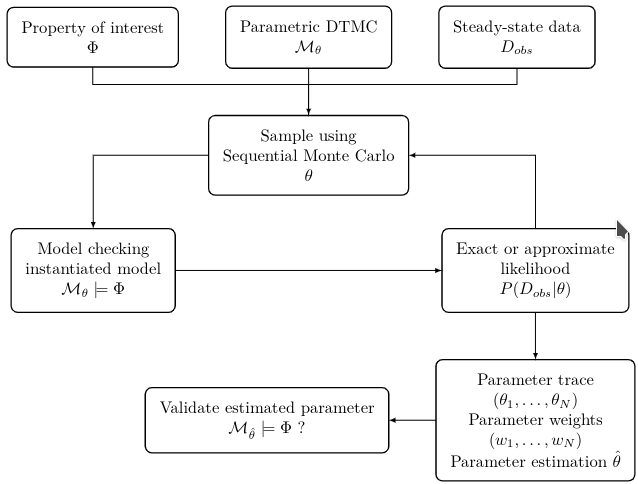
\includegraphics[width=0.7\textwidth]{figures/bbeess-framework.png}
        \caption{Generic framework for Bayesian parameter synthesis of parametric DTMC.}
        \label{fig:generic-framework}
    \end{figure}
\end{frame}

\begin{frame}
    \frametitle{Generic framework}
    \begin{itemize}
        \item Input:
              \begin{itemize}
                  \item $\mathcal{M}_\theta$: parametric DTMC of parameter $\theta$
                  \item $\Phi$: bounded reachability property of interest.
                  \item $D_{obs}$: observed data.
                  \item $N$: number of particles.
              \end{itemize}
        \item Output:
              \begin{itemize}
                  \item $(\theta_1,\ldots,\theta_{N_{MH}})$, sampled particles
                  \item $(w_1,\ldots,w_{N_{MH}})$ particle corresponding weights.
                  \item $\hat{p}=P(\mathcal{M}_{\hat{\theta}}\models\Phi)$
              \end{itemize}
    \end{itemize}
\end{frame}

\begin{frame}
    \frametitle{Generic framework}
    \footnotesize{
        \begin{algorithm}[H]
            \caption{Generic framework for Bayesian parameter synthesis}
            \label{alg:generic-framework}
            \begin{algorithmic}[1]
                \Procedure{Generic-Bayesian-Monte-Carlo}{}
                \State $i \leftarrow 1$
                \While{$i \leq N$}
                \State Sample $\theta$ with corresponding weight $w$
                \NoNumber{\hspace{1.5cm} by Sequential Monte Carlo sampling algorithm.}
                \State Verify instantiated model $\mathcal{M}_\theta$ against $\Phi$
                \If{$\mathcal{M}_\theta \models \Phi$}
                \State $\theta_i \leftarrow \theta$
                \State Estimate $w_i$ as exact or approximated likelihood $P(D_{obs}|\theta)$
                \EndIf
                \EndWhile
                \State Estimate $\hat{\theta}$ using posterior mean.
                \State Compute $\hat{p}=P(\mathcal{M}_{\hat{\theta}}\models\Phi)$
                \State Return $(\theta_1,\ldots,\theta_{N})$, $(w_1,\ldots,w_{N})$, $\hat{\theta}$, $\hat{p}$
                \EndProcedure
            \end{algorithmic}
        \end{algorithm}
    }
\end{frame}

\begin{frame}
    \frametitle{RF-SMC}
    \begin{itemize}
        \item Based on Sequential Monte-Carlo
        \item Model checking using precomputed symbolic reachability probability at each SMC
              perturbation step.
              \begin{itemize}
                  \item At each MH transition, a particle is accepted only if it instantiates a
                        satisfying model.
              \end{itemize}
    \end{itemize}
\end{frame}

\begin{frame}
    \frametitle{RF-SMC}
    \footnotesize{
        \begin{algorithm}[H]
            \caption{Metropolis-Hastings with rational functions}
            \label{alg:rf-mh}
            \begin{algorithmic}[1]
                \Procedure{RF-MH}{}
                \State Init empty trace $T$
                \State Draw $\theta_{cand}$ from $\pi(\theta)$ s.t $\mathcal{M}_{\theta_{cand}}\models\Phi$ (evaluating $RF_{\Phi}(\theta)$)
                \State Append $\theta_{cand}$ to trace $T$
                \State $i \leftarrow 2$
                \While{$i \leq N_{MH}$}
                \State Draw $\theta_{cand}$ from $Q(\theta'|\theta_{i-1})$ s.t $\mathcal{M}_{\theta_{cand}}\models\Phi$ (evaluating $RF_{\Phi}(\theta)$)
                \State Evaluate $\xi = \min(0, \ln(P(D_{obs}|\theta_{cand})) - \ln(P(D_{obs}|\theta_{i-1}))) > 0$
                \If{$\xi > 0$}
                \State Append $\theta_{cand}$ to trace $T$
                \Else
                \State Draw a random number $u$ from $Uniform(0,1)$
                \If{$u \leq \exp(\xi)$}
                \State Append $\theta_{cand}$ to trace $T$
                \EndIf
                \EndIf
                \EndWhile
                \State Return $(\theta_1,\ldots,\theta_{N_{MH}})$, $(w_1,\ldots,w_{N_{MH}})$
                \EndProcedure
            \end{algorithmic}
        \end{algorithm}
    }
\end{frame}

\begin{frame}
    \frametitle{RF-SMC}
    \footnotesize{
        \begin{algorithm}[H]
            \caption{Sequential Monte Carlo with rational functions}
            \label{alg:rf-smc}
            \begin{algorithmic}[1]
                \Procedure{RF-SMC}{}
                \State Draw $(\theta_1,\ldots,\theta_N)$ from $\pi(\theta)$ s.t $\mathcal{M}_{\theta_i}\models\Phi$ (evaluating $RF_{\Phi}(\theta)$)
                \State $t \leftarrow 1$
                \While{$t \leq M$}
                \State Normalize $(w^{t-1}_1,\ldots,w^{t-1}_N)$  \algorithmiccomment{SMC correction step}
                \State Sample with replacement $(\theta^t_1,\ldots,\theta^t_N)$ \algorithmiccomment{SMC selection step}
                \NoNumber{\hspace{.5cm}} from $(\theta^{t-1}_1,\ldots,\theta^{t-1}_N)$ with probabilities $(w^{t-1}_1,\ldots,w^{t-1}_N)$
                \State $i \leftarrow 1$
                \While{$i \leq N$} \algorithmiccomment {SMC perturbation step}
                \State Draw $\hat{\theta}^t_i$ from $F_t(\theta^t | \theta^{t-1}_1,\ldots,\theta^{t-1}_N), 1\leq t \leq M$
                \State Mutate $(\theta^*_1,\ldots,\theta^*_{N_{MH}}), (w^*_1,\ldots,w^*_{N_{MH}}) \leftarrow RF-MH(\hat{\theta}^t_i)$
                \State $\theta_i, w_i \leftarrow \theta^*_{N_{MH}}, w^*_{N_{MH}}$
                \EndWhile
                \EndWhile
                \State Estimate $\hat{\theta}$ using posterior mean, compute $\hat{p}=P(\mathcal{M}_{\hat{\theta}}\models\Phi)$
                \State Return $(\theta_1,\ldots,\theta_{N})$, $(w_1,\ldots,w_{N})$, $\hat{\theta}$, $\hat{p}$
                \EndProcedure
            \end{algorithmic}
        \end{algorithm}
    }
\end{frame}

\begin{frame}
    \frametitle{SMC-ABC-SMC}
    Without the availability of analytical form to evaluate the steady-state distribution and the property of
    interest, we face the following obstacles:
    \begin{itemize}
        \item \textbf{Absence of likelihood functions}
              \begin{itemize}
                  \item no analytical form of likelihood.
                  \item $\Rightarrow$ likelihood-free methods (Approximate Bayesian Computation)
              \end{itemize}
        \item \textbf{Absence of rational functions for evaluation of property of interest}
              \begin{itemize}
                  \item $\Rightarrow$ Statistical model checking
              \end{itemize}
    \end{itemize}
\end{frame}

\begin{frame}
    \frametitle{SMC-ABC-SMC}
    \footnotesize{
        \begin{algorithm}[H]
            \caption{Sequential Monte-Carlo with simulations}
            \label{alg:smc-abc-smc}
            \begin{algorithmic}[1]
                \Procedure{SMC-ABC-SMC}{}
                \State Draw $(\theta_1,\ldots,\theta_N)$ from $\pi(\theta)$ s.t $\mathcal{M}_{\theta_i}\models\Phi$ (Statistical MC)
                \State $t \leftarrow 1$
                \While{$t \leq M$}
                \State Normalize $(w^{t-1}_1,\ldots,w^{t-1}_N)$  \algorithmiccomment{SMC correction step}
                \State Sample with replacement $(\theta^t_1,\ldots,\theta^t_N)$ \algorithmiccomment{SMC selection step}
                \NoNumber{\hspace{.5cm}} from $(\theta^{t-1}_1,\ldots,\theta^{t-1}_N)$ with probabilities $(w^{t-1}_1,\ldots,w^{t-1}_N)$
                \State $i \leftarrow 1$
                \While{$i \leq N$} \algorithmiccomment {SMC perturbation step}
                \State Draw $\hat{\theta}^t_i$ from $F_t(\theta^t | \theta^{t-1}_1,\ldots,\theta^{t-1}_N), 1\leq t \leq M$
                \If{Statistical Model Checking $\mathcal{M}_{\hat{\theta}^t_i} \models \Phi$}
                \State Simulate $D_{sim}$ from $\mathcal{M}_{\hat{\theta}^t_i}$
                \If{$\delta = Distance(D_{sim}, D_{obs}) < \epsilon)$}
                \State $\theta_i, w_i \leftarrow \hat{\theta}^t_i, \delta^{-1}$
                \EndIf
                \EndIf
                \EndWhile
                \EndWhile
                \State Estimate $\hat{\theta}$ using posterior mean, compute $\hat{p}=P(\mathcal{M}_{\hat{\theta}}\models\Phi)$
                \State Return $(\theta_1,\ldots,\theta_{N})$, $(w_1,\ldots,w_{N})$, $\hat{theta}$, $\hat{p}$
                \EndProcedure
            \end{algorithmic}
        \end{algorithm}
    }
\end{frame}

\begin{frame}
    \frametitle{Comparison}
    \begin{figure}[H]
        \centering
        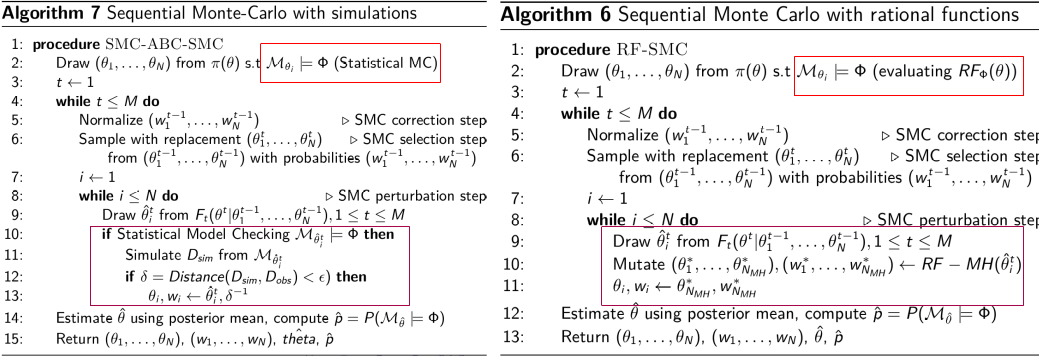
\includegraphics[width=\textwidth]{figures/smc-compare.png}
        \caption{Comparison between RF-SMC and SMC-ABC-SMC.}
        \label{fig:comparison}
    \end{figure}
\end{frame}


%%%%%%%%%%%%%%%%%%%%%%%%%%%%%%%%%%%%%%%%%%%%%%%%%%%%%%%%%%%%%%%%%%%%%%%%%%%%%%%%%%%%%%%%%%%%%%%%%%%%
\section{Evaluation}
\begin{frame}
    \begin{center}
        \Huge Evaluation
    \end{center}
\end{frame}

\begin{frame}
    \frametitle{Evaluation}
    Case studies:
    \begin{itemize}
        \item Zeroconf
        \item Social feedback in honeybee colonies
        \item SIR
    \end{itemize}
    Evaluation environment:
    \begin{itemize}
        \item Hardware: Intel Xeon W-2135, 64GB RAM
        \item OS: OpenSUSE 15.2
        \item Libraries: Storm @stable, PRISM 4.6, Python 3.8.8
    \end{itemize}
\end{frame}

\begin{frame}
    \frametitle{Zeroconf}
    Zero-configuration protocol (\textit{zeroconf} for short) \cite{ZeroConf} is a protocol used in
    IPv4 network to allocate newly attached device an unique IP address without any intervention
    from network operators.
    \begin{figure}[H]
        \centering
        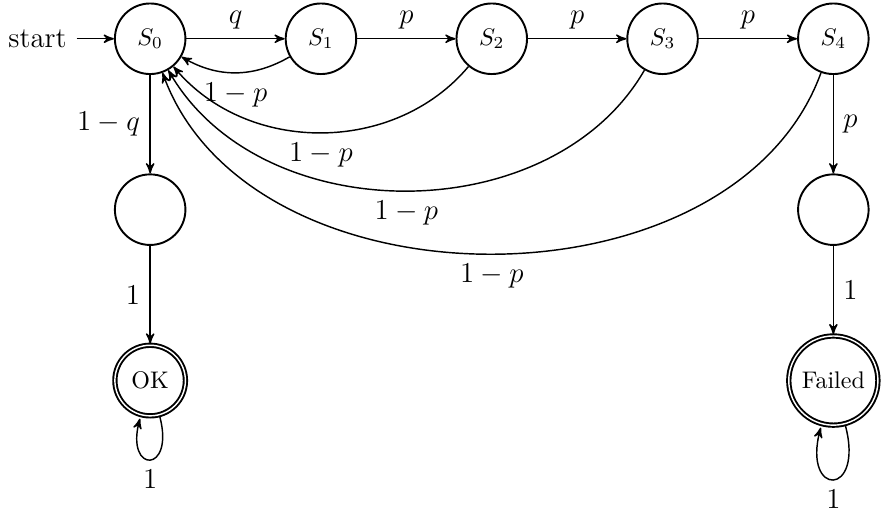
\includegraphics[width=0.8\textwidth]{figures/zeroconf4_dtmc.png}
        \caption{Example of an IPv4 Zeroconf model with 4 probes}
        \label{fig:zeroconf4}
    \end{figure}
\end{frame}

\begin{frame}
    \frametitle{Zeroconf}
    We select a true parameter $(p, q)$ arbitrarily random for Zeroconf model of 4 and 10 states.
    \footnotesize{
        \begin{table}[H]
            \begin{tabular}{|l|l|l|}
                \hline
                Model $\mathcal{M}$        & Zeroconf, 4 probes                                                  & Zeroconf, 10 probes                                                  \\ \hline
                Number of BSCCs            & 2                                                                   & 2                                                                    \\ \hline
                Number of states           & 9                                                                   & 14                                                                   \\ \hline
                \begin{tabular}[c]{@{}l@{}}True parameter\\ $\theta=(p,q)$ \end{tabular} & (0.105547, 0.449658)                                                & (0.197779, 0.621824)                                                 \\ \hline
                Number of samples          & 10000                                                               & 10000                                                                \\ \hline
                \begin{tabular}[c]{@{}l@{}}Synthetic data\\ $D_{obs}$ \end{tabular} & (41, 9959)                                                          & (22, 9978)                                                           \\ \hline
                \begin{tabular}[c]{@{}l@{}}Property of interest\\ $\Phi$ \end{tabular} & $P_{\geq 0.75} (\texttt{true} \mathsf{U}^{\leq 4} (\texttt{"OK"}))$ & $P_{\geq 0.75} (\texttt{true} \mathsf{U}^{\leq 10} (\texttt{"OK"}))$ \\ \hline
                \begin{tabular}[c]{@{}l@{}}Satisfaction property\\ $P(\mathcal{M}_\theta\models\Phi)$\end{tabular} & 0.946409                                                            & 0.952067                                                             \\ \hline
            \end{tabular}
            \caption{Synthetic data for Zeroconf model of 4 and 10 probes.}
        \end{table}
    }
\end{frame}

\begin{frame}
    \frametitle{Zeroconf 4 results}
    \footnotesize{
        \begin{table}[H]
            \begin{tabular}{|l|l|l|}
                \hline
                Method                                           & RF-SMC               & SMC-ABC-SMC          \\ \hline
                Estimated parameter $\hat{\theta}$               & (0.188956, 0.460554) & (0.176469, 0.355322) \\ \hline
                True parameter $\theta$                          & (0.105547, 0.449658) & (0.105547, 0.449658) \\ \hline
                L2 distance $\Vert \theta, \hat{\theta} \Vert_2$ & 0.084117             & 0.118023             \\ \hline
                $P(\mathcal{M}_{\hat{\theta}}\models\Phi)$       & 0.893715             & 0.918133             \\ \hline
            \end{tabular}
            \caption{Parameter estimation results for Zeroconf model of 4 probes.}
        \end{table}
    }
\end{frame}

\begin{frame}
    \frametitle{Zeroconf 4 results}
    \begin{figure}[H]
        \centering
        \begin{subfigure}{0.48\textwidth}
            \centering
            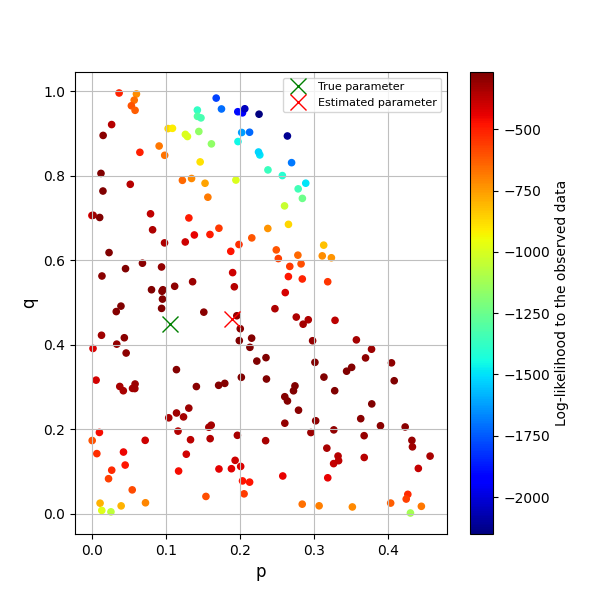
\includegraphics[width=\linewidth]{figures/zeroconf4_rf.png}
            \caption{Sampled particles using Rational Functions SMC}
        \end{subfigure}
        \hfill
        \begin{subfigure}{0.48\textwidth}
            \centering
            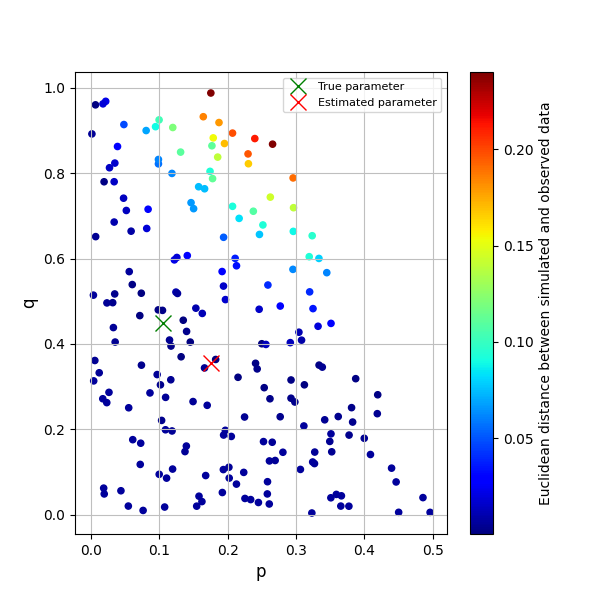
\includegraphics[width=\linewidth]{figures/zeroconf4_sim.png}
            \caption{Sampled particles using Statiscal Model Checking ABC-SMC}
        \end{subfigure}
        \caption{Parameter synthesis results for Zeroconf model of 4 probes.}
    \end{figure}
\end{frame}


\begin{frame}
    \frametitle{Zeroconf 4 results}
    Runtime
    \begin{table}[H]
        \centering
        \begin{tabular}{|l|l|l|}
            \hline
            Method                     & RF-SMC & SMC-ABC-SMC \\ \hline
            Total runtime (minutes)    & 6.083  & 54.867      \\ \hline
            \begin{tabular}[c]{@{}l@{}}Average perturbation\\ runtime (minutes)\end{tabular} & 0.32   & 2.88        \\ \hline
        \end{tabular}
        \caption{Physical runtime on Zeroconf model with 4 probes.}
    \end{table}
\end{frame}


\begin{frame}
    \frametitle{Zeroconf 10 results}
    \footnotesize{
        \begin{table}[H]
            \begin{tabular}{|l|l|l|}
                \hline
                Method                                           & RF-SMC               & SMC-ABC-SMC          \\ \hline
                True parameter $\theta$                          & (0.197779, 0.621824) & (0.197779, 0.621824) \\ \hline
                Estimated parameter $\hat{\theta}$               & (0.301807, 0.457090) & (0.378774, 0.405870) \\ \hline
                L2 distance $\Vert \theta, \hat{\theta} \Vert_2$ & 0.194831             & 0.281772             \\ \hline
                $P(\mathcal{M}_{\hat{\theta}}\models\Phi)$       & 0.952067             & 0.966142             \\ \hline
            \end{tabular}
            \caption{Parameter estimation results for Zeroconf model of 10 probes.}
        \end{table}
    }
\end{frame}

\begin{frame}
    \frametitle{Zeroconf 10 results}
    \begin{figure}[H]
        \centering
        \begin{subfigure}{0.48\textwidth}
            \centering
            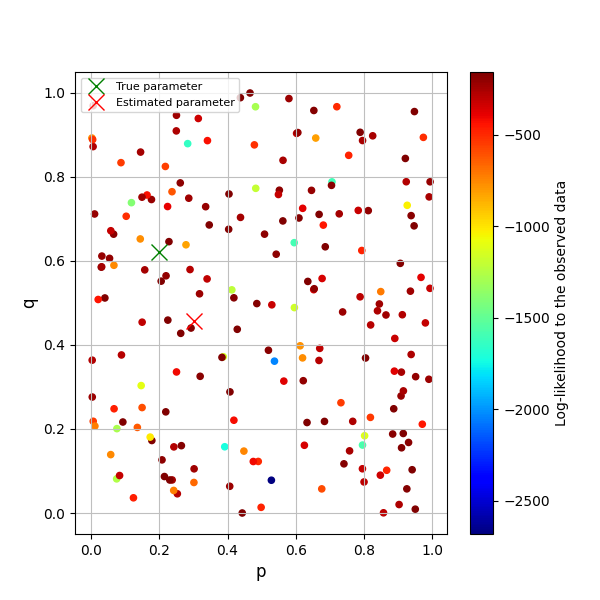
\includegraphics[width=\linewidth]{figures/zeroconf10_rf.png}
            \caption{Sampled particles using RF-SMC}
        \end{subfigure}
        \hfill
        \begin{subfigure}{0.48\textwidth}
            \centering
            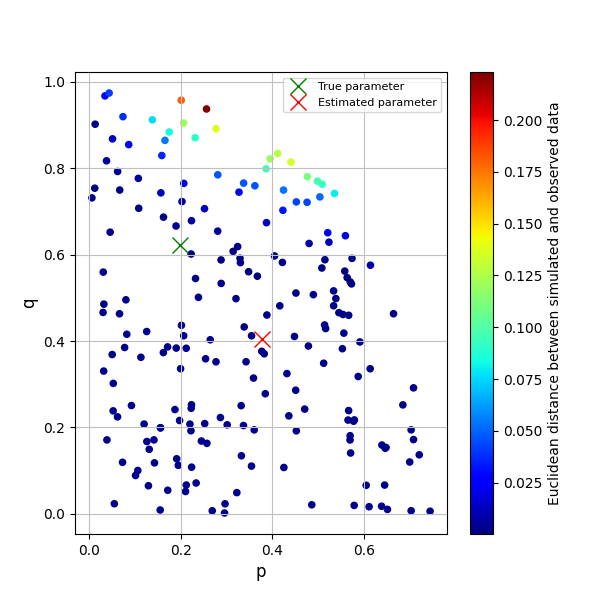
\includegraphics[width=\linewidth]{figures/zeroconf10_sim.png}
            \caption{Sampled particles using SMC-ABC-SMC}
        \end{subfigure}
        \caption{Parameter synthesis results for Zeroconf model of 10 probes.}
    \end{figure}
\end{frame}

\begin{frame}
    \frametitle{Zeroconf 10 results}
    Runtime
    \begin{table}[H]
        \centering
        \begin{tabular}{|l|l|l|}
            \hline
            Method                     & RF-SMC & SMC-ABC-SMC \\ \hline
            Total runtime (minutes)    & 9.50   & 37.93       \\ \hline
            \begin{tabular}[c]{@{}l@{}}Average perturbation\\ runtime (minutes)\end{tabular} & 0.501  & 1.978       \\ \hline
        \end{tabular}
        \caption{Physical runtime on Zeroconf model with 10 probes.}
    \end{table}
\end{frame}


\begin{frame}
    \frametitle{Zeroconf results discussion}
    \begin{figure}[H]
        \centering
        \begin{subfigure}{0.3\textwidth}
            \centering
            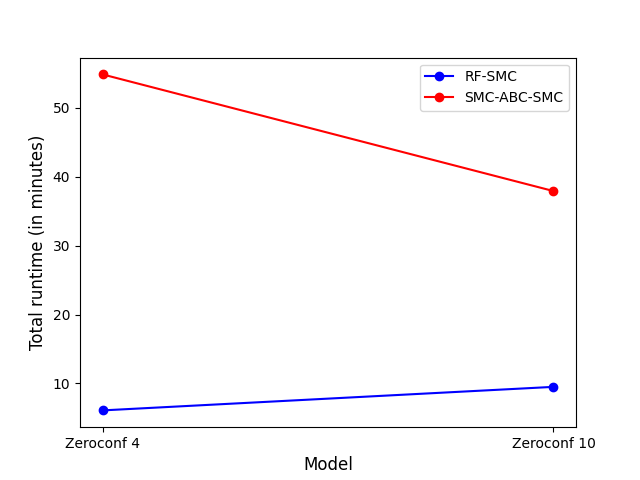
\includegraphics[width=\linewidth]{figures/zeroconf_runtime_total.png}
            \caption{Total runtime}
        \end{subfigure}
        \hfill
        \begin{subfigure}{0.3\textwidth}
            \centering
            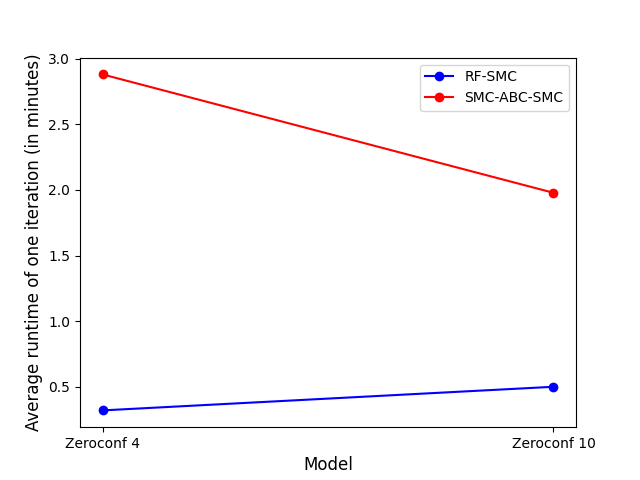
\includegraphics[width=\linewidth]{figures/zeroconf_runtime_avg.png}
            \caption{Average perturbation runtime}
        \end{subfigure}
        \caption{Physical runtime on Zeroconf model of different sizes.}
    \end{figure}
    \begin{itemize}
        \item RF-SMC and SMC-ABC-SMC have similar accuracy.
        \item RF-SMC is much faster
    \end{itemize}
\end{frame}

\begin{frame}
    \frametitle{Social feedback in honeybee colonies}
    Each bee in a colony possibly stings after observing a threat in the surrounding environment and
    warns other bees by releasing a special substance, pheromone. There are 3 assumptions on the system:
    \begin{enumerate}
        \item Each bee releases a unit amount of pheromone immediately after stinging.
        \item A bee dies after stinging and releasing a pheromone unit. In other words, no bee can sting
              more than once.
        \item Stinging behavior only depends on the concentration of pheromone in the environment.
    \end{enumerate}
\end{frame}

\begin{frame}
    \frametitle{Social feedback in honeybee colonies}
    \begin{figure}[H]
        \centering
        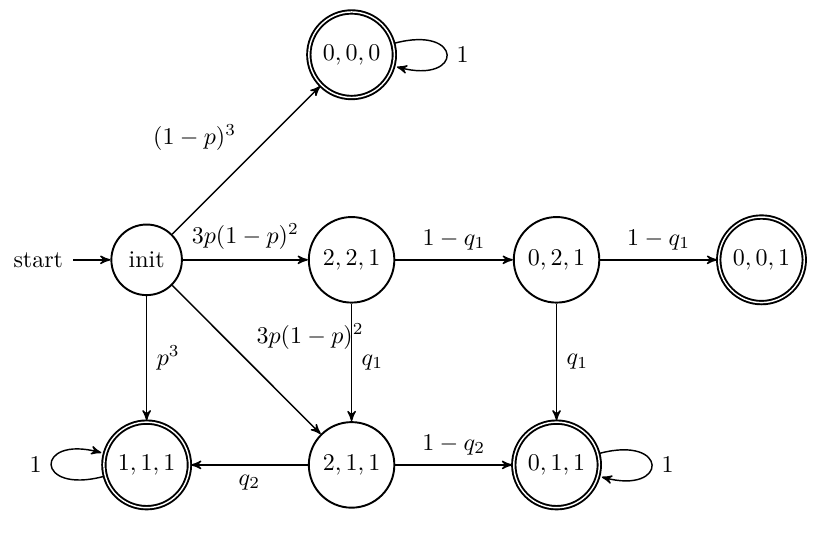
\includegraphics[width=0.8\textwidth]{figures/bees-dtmc.png}
        \caption{Parametric DTMC model of 3 bees with 3 parameters $p, q_1, q_2$}
        \label{fig:bees3}
    \end{figure}
\end{frame}

\begin{frame}
    \frametitle{Social feedback in honeybee colonies}
    True parameters and synthetic data.
    \begin{table}[H]
        \tiny
        \centering
        \begin{tabular}{|l|l|l|l|}
            \hline
            Model $\mathcal{M}$                & 3 bees                                         & 5 bees                                           & 10 bees                                          \\ \hline
            Number of states                   & 13                                             & 24                                               & 69                                               \\ \hline
            Number of BSCCs                    & 4                                              & 6                                                & 11                                               \\ \hline
            True parameter $\theta$            & \begin{tabular}[c]{@{}l@{}}$p=0.665623$ \\ $q_1=0.830401$ \\ $q_2=0.839778$ \end{tabular}                     & \begin{tabular}[c]{@{}l@{}}$p=0.278370$ \\ $q_1=0.305994$ \\ $q_2=0.489792$ \\ $q_3=0.737252$ \\ $q_4=0.766581$ \end{tabular}                       & \begin{tabular}[c]{@{}l@{}}$p=0.222169$ \\ $q_1=0.246993$ \\ $q_2=0.281934$ \\ $q_3=0.446384$ \\ $q_4=0.491612$ \\ $q_5=0.534611$ \\ $q_6=0.569409$ \\ $q_7=0.684651$ \\ $q_8=0.717139$ \\ $q_9=0.800987$  \end{tabular}                       \\ \hline
            Synthetic data $D_{obs}$           & (344, 54, 1390, 8212)                          & \begin{tabular}[c]{@{}l@{}}(1940, 11, 216, \\ 2682, 4200, 951)\end{tabular}                       & \begin{tabular}[c]{@{}l@{}}(769, 0, 1, 10, 187, 972,\\  2494, 2982, 2133, 419, 33)\end{tabular}                       \\ \hline
            Target property $\Phi$             & $P_{\geq 0.25} (\text{true} \mathsf{U} (S>3))$ & $P_{\geq 0.25} (\texttt{true} \mathsf{U} (S>5))$ & $P_{\geq 0.25} (\texttt{true} \mathsf{U} (S>8))$ \\ \hline
            $P(\mathcal{M}_\theta\models\Phi)$ & 0.819666                                       & 0.780172                                         & 0.737244                                         \\ \hline
        \end{tabular}
        \caption{True parameter and synthetic data for 3, 5, and 10 bees models.}
    \end{table}
\end{frame}

\begin{frame}
    \frametitle{Social feedback in honeybee colonies}
    \begin{table}[H]
        \centering
        \footnotesize
        \begin{tabular}{|l|l|l|}
            \hline
                                                              & RF-SMC                     & SMC-ABC-SMC                \\ \hline
            True parameter $\theta$                           & \begin{tabular}[c]{@{}l@{}}$p=0.665623$ \\ $q_1=0.830401$ \\ $q_2=0.839778$ \end{tabular} & \begin{tabular}[c]{@{}l@{}}$p=0.665623$ \\ $q_1=0.830401$ \\ $q_2=0.839778$ \end{tabular} \\ \hline
            Estimated parameter $\hat{\theta}$                & \begin{tabular}[c]{@{}l@{}}$p=0.671388$ \\ $q_1=0.575026$ \\ $q_2=0.525502$ \end{tabular} & \begin{tabular}[c]{@{}l@{}}$p=0.811651$ \\ $q_1=0.621073$ \\ $q_2=0.544130$ \end{tabular} \\ \hline
            L2 distance  $\Vert \theta, \hat{\theta} \Vert_2$ & 0.404992                   & 0.390576                   \\ \hline
            $P(\mathcal{M}_{\hat{\theta}}\models\Phi)$        & 0.623889                   & 0.595083                   \\ \hline
        \end{tabular}
        \caption{Parameter synthesis result for 3 bees model.}
    \end{table}
\end{frame}

\begin{frame}
    \frametitle{Social feedback in honeybee colonies}
    \begin{table}[H]
        \centering
        \footnotesize
        \begin{tabular}{|l|l|l|}
            \hline
            Method                     & RF-SMC & SMC-ABC-SMC \\ \hline
            Total runtime (minutes)    & 5.917  & 68.783      \\ \hline
            \begin{tabular}[c]{@{}l@{}}Average perturbation\\ runtime (minutes)\end{tabular} & 0.312  & 3.614       \\ \hline
        \end{tabular}
        \caption{Physical runtime on 3 bees model.}
    \end{table}
\end{frame}

\begin{frame}
    \frametitle{Social feedback in honeybee colonies}
    \begin{table}[H]
        \centering
        \footnotesize
        \begin{tabular}{|l|l|l|}
            \hline
                                                              & RF-SMC                      & SMC-ABC-SMC                 \\ \hline
            True parameter $\theta$                           & \begin{tabular}[c]{@{}l@{}}$p=0.278370$ \\ $q_1=0.305994$ \\ $q_2=0.489792$ \\ $q_3=0.737252$ \\ $q_4=0.766581$ \end{tabular}  & \begin{tabular}[c]{@{}l@{}}$p=0.278370$ \\ $q_1=0.305994$ \\ $q_2=0.489792$ \\ $q_3=0.737252$ \\ $q_4=0.766581$ \end{tabular}  \\ \hline
            Estimated parameter $\hat{\theta}$                & \begin{tabular}[c]{@{}l@{}}$p=0.576565$ \\ $q_1=0.589724$ \\ $q_2=0.490334$ \\ $q_3=0.554397$ \\ $q_4=0.524433$ \end{tabular} & \begin{tabular}[c]{@{}l@{}}$p=0.361220$ \\ $q_1=0.316007$ \\ $q_2=0.545691$ \\ $q_3=0.643962$ \\ $q_4=0.591206$ \end{tabular} \\ \hline
            L2 distance  $\Vert \theta, \hat{\theta} \Vert_2$ & 0.511366                    & 0.222594                    \\ \hline
            $P(\mathcal{M}_{\hat{\theta}}\models\Phi)$        & 0.623889                    & 0.595083                    \\ \hline
        \end{tabular}
        \caption{Parameter synthesis result for 5 bees model}
    \end{table}
\end{frame}

\begin{frame}
    \frametitle{Social feedback in honeybee colonies}
    \begin{table}[H]
        \centering
        \footnotesize
        \begin{tabular}{|l|l|l|}
            \hline
            Method                      & RF-SMC & SMC-ABC-SMC \\ \hline
            Total runtime (minutes)     & 29.517 & 352.083     \\ \hline
            \begin{tabular}[c]{@{}l@{}}Average perturbation\\ runtime (minutes)\end{tabular} & 1.553  & 18.518      \\ \hline
        \end{tabular}
        \caption{Physical runtime on 5 bees model.}
    \end{table}
\end{frame}


\begin{frame}
    \frametitle{Social feedback in honeybee colonies}
    \begin{table}[H]
        \centering
        \tiny
        \begin{tabular}{|l|l|l|}
            \hline
                                                              & RF-SMC                      & SMC-ABC-SMC                 \\ \hline
            True parameter $\theta$                           & \begin{tabular}[c]{@{}l@{}}$p=0.222169$ \\ $q_1=0.246993$ \\ $q_2=0.281934$ \\ $q_3=0.446384$ \\ $q_4=0.491612$ \\ $q_5=0.534611$ \\ $q_6=0.569409$ \\ $q_7=0.684651$ \\ $q_8=0.717139$ \\ $q_9=0.800987$  \end{tabular} & \begin{tabular}[c]{@{}l@{}}$p=0.222169$ \\ $q_1=0.246993$ \\ $q_2=0.281934$ \\ $q_3=0.446384$ \\ $q_4=0.491612$ \\ $q_5=0.534611$ \\ $q_6=0.569409$ \\ $q_7=0.684651$ \\ $q_8=0.717139$ \\ $q_9=0.800987$  \end{tabular} \\ \hline
            Estimated parameter $\hat{\theta}$                & \begin{tabular}[c]{@{}l@{}}$p=0.604881$ \\ $q_1=0.472557$ \\ $q_2=0.281484$ \\ $q_3=0.500706$ \\ $q_4=0.49340$ \\ $q_5=0.495508$ \\ $q_6=0.466596$ \\ $q_7=0.510167$ \\ $q_8=0.474153$ \\ $q_9=0.484061$  \end{tabular} & \begin{tabular}[c]{@{}l@{}}$p=0.391313$ \\ $q_1=0.485688$ \\ $q_2=0.424056$ \\ $q_3=0.381489$ \\ $q_4=0.440681$ \\ $q_5=0.578865$ \\ $q_6=0.594232$ \\ $q_7=0.564557$ \\ $q_8=0.547804$ \\ $q_9=0.520006$  \end{tabular} \\ \hline
            L2 distance  $\Vert \theta, \hat{\theta} \Vert_2$ & 0.665837                    & 0.487042                    \\ \hline
            $P(\mathcal{M}_{\hat{\theta}}\models\Phi)$        & 0.933287                    & 0.907478                    \\ \hline
        \end{tabular}
        \caption{Parameter synthesis result for 10 bees model}
    \end{table}
\end{frame}

\begin{frame}
    \frametitle{Social feedback in honeybee colonies}
    \begin{table}[H]
        \centering
        \footnotesize
        \begin{tabular}{|l|l|l|}
            \hline
            Method                      & RF-SMC   & SMC-ABC-SMC \\ \hline
            Total runtime (minutes)     & 3976.117 & 581.833     \\ \hline
            \begin{tabular}[c]{@{}l@{}}Average perturbation\\ runtime (minutes)\end{tabular} & 209.237  & 30.592      \\ \hline
        \end{tabular}
        \caption{Physical runtime on 10 bees model.}
    \end{table}
\end{frame}


\begin{frame}
    \frametitle{Social feedback in honeybee colonies}
    \begin{figure}[H]
        \centering
        \begin{subfigure}{0.3\textwidth}
            \centering
            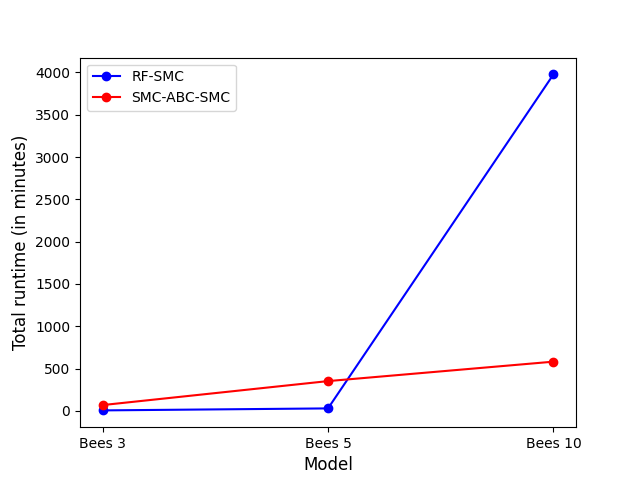
\includegraphics[width=\linewidth]{figures/bees_runtime_total.png}
            \caption{Total runtime}
        \end{subfigure}
        \hfill
        \begin{subfigure}{0.3\textwidth}
            \centering
            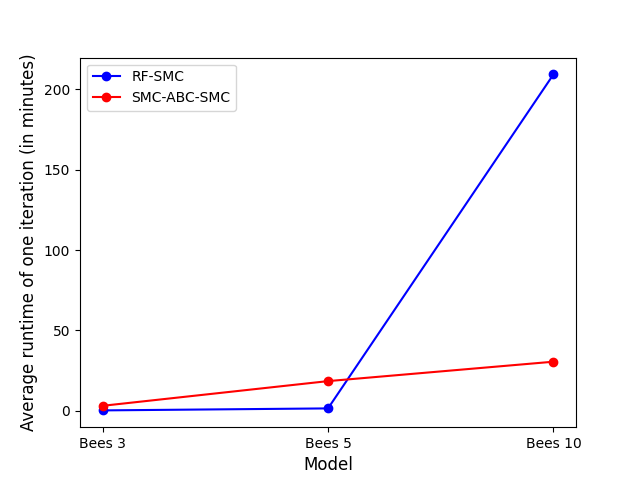
\includegraphics[width=\linewidth]{figures/bees_runtime_avg.png}
            \caption{Average perturbation runtime}
        \end{subfigure}
        \caption{Physical runtime on bees model of different sizes.}
    \end{figure}
    Results discussion
    \begin{itemize}
        \item SMC-ABC-SMC delivers results with higher accuracy and comparable satisfaction probability.
        \item From 10 bees model, RF-SMC becomes much slower than SMC-ABC-SMC.
    \end{itemize}
\end{frame}

\begin{frame}
    \frametitle{SIR}
    \textit{SIR} model (Kermack \cite{kermack1927contribution}) is a model widely used in modeling
    epidemics. In a \text{SIR} model, each individual is of one among three types:
    \begin{itemize}
        \item \textit{Susceptible (S)}
        \item \textit{Infected (I)}
        \item \textit{Recovered (R)}
    \end{itemize}
    SIR is a stochastic system modeled by reactions between $S$, $I$ and $R$. In this thesis, we use
    only two reactions.
    \begin{align*}
        R_1: & S + I \xrightarrow{\alpha} 2I \\
        R_2: & I     \xrightarrow{\beta} R
    \end{align*}
\end{frame}

\begin{frame}
    \frametitle{SIR}
    Reactions $R_1, R_2$ generate continuous-time Markov chain (CTMC) depends on the initital population
    \begin{figure}[H]
        \centering
        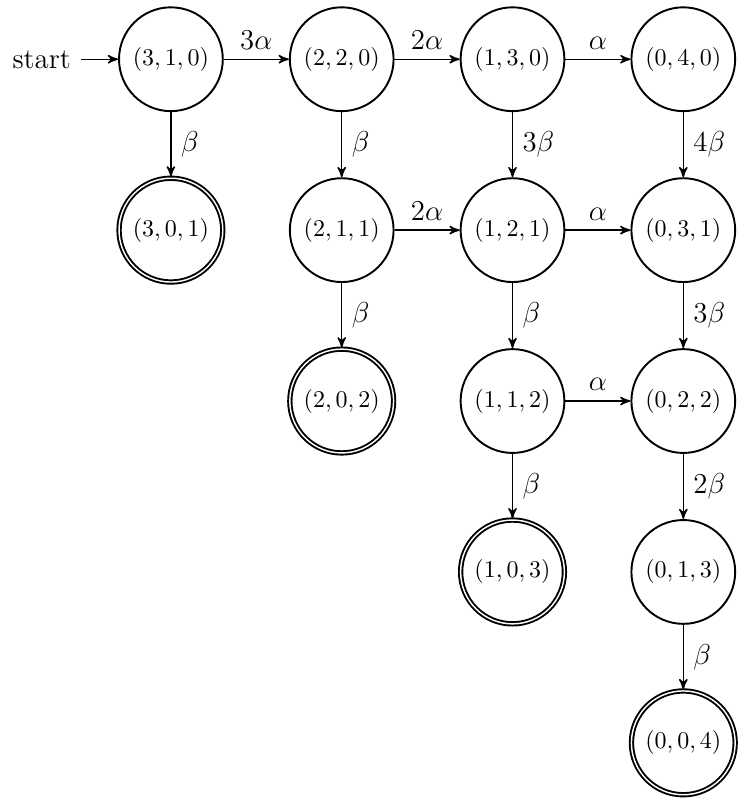
\includegraphics[width=0.5\linewidth]{figures/sir310_ctmc.png}
        \caption{$SIR(3,1,0)$ CTMC model with parameters$(\alpha, \beta)$.}
    \end{figure}
\end{frame}

\begin{frame}
    \frametitle{SIR}
    We uniformize CTMC into DTMC
    \begin{figure}[H]
        \centering
        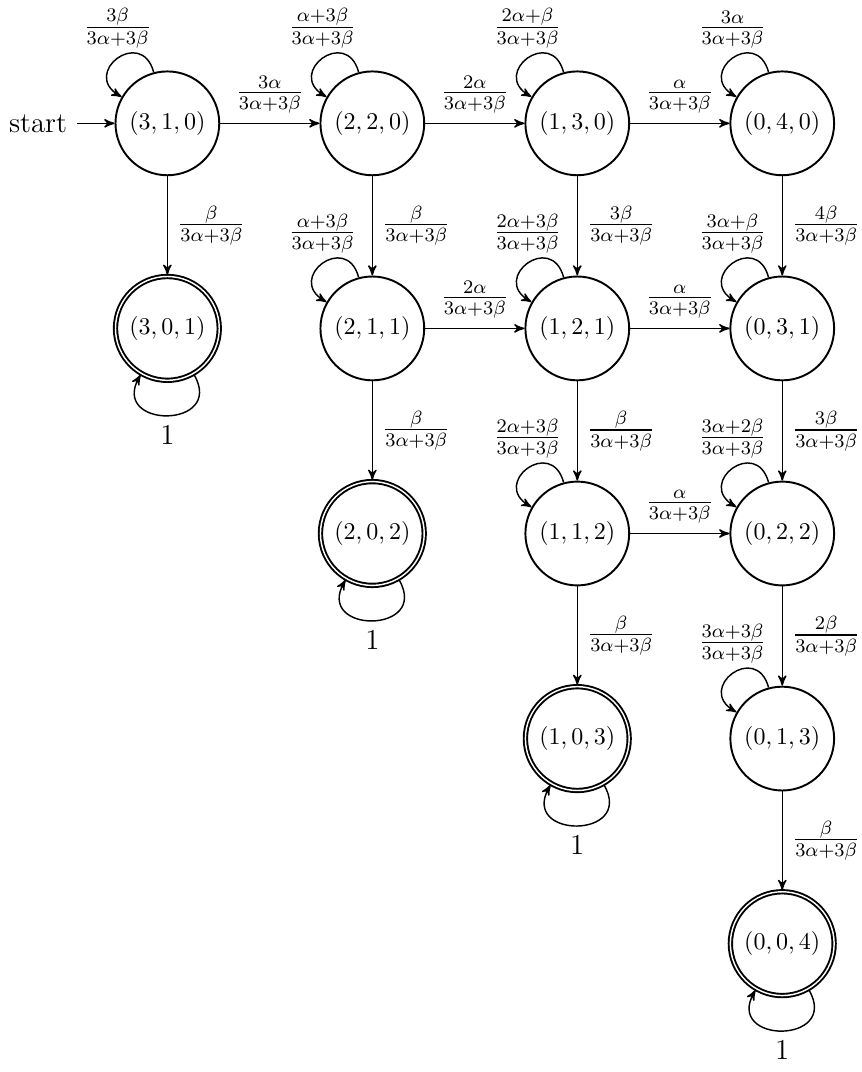
\includegraphics[width=0.5\linewidth]{figures/sir310_dtmc.png}
        \caption{$SIR(3,1,0)$ uniformized DTMC model with  uniformization rate $(3\alpha + 4\beta)$.}
    \end{figure}
\end{frame}

\begin{frame}
    \frametitle{SIR}
    As uniformization of a CTMC preserves bounded until properties, we conduct parameter synthesis
    experiments on uniformized DTMC. We verify the following property
    \begin{block}{SIR property of interest}
        "With the probability of
        at least 25 percent, the number of infected individuals does not exceed half of the population until
        the system is in its steady-state. Let $N=S_0+I_0+R_0$. In the PCTL formula we have:
        \begin{align*}
            P_{\geq 0.25} ( !(i > N/2) \quad \mathsf{U}^{\leq N} \quad (i = 0) )
        \end{align*}
    \end{block}
\end{frame}

\begin{frame}
    \frametitle{SIR}
    \begin{figure}[H]
        \centering
        \begin{subfigure}{0.4\textwidth}
            \centering
            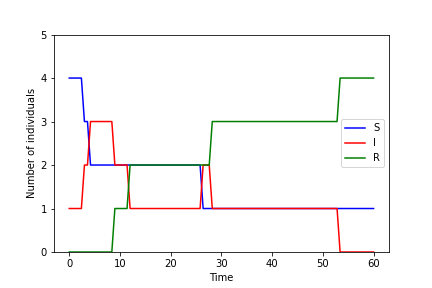
\includegraphics[width=\linewidth]{figures/sir_510_trace_1.png}
            \caption{Example with SIR(5,1,0)}
        \end{subfigure}
        \hfill
        \begin{subfigure}{0.4\textwidth}
            \centering
            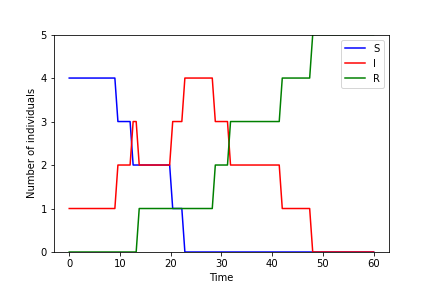
\includegraphics[width=\linewidth]{figures/sir_510_trace_2.png}
            \caption{Counter-example with SIR(5,1,0)}
        \end{subfigure}
        \caption{Example and counter-example on SIR(5,1,0) CTMC with $(\alpha, \beta)=(0.034055, 0.087735)$.}
    \end{figure}
\end{frame}

\begin{frame}
    \frametitle{SIR}
    \begin{table}[H]
        \tiny
        \begin{tabular}{|l|l|l|l|}
            \hline
            Model $\mathcal{M}$                          & SIR(5,1,0)                                          & SIR(10,1,0)                                          & SIR(15,1,0)                                          \\ \hline
            Number of BSCCs                              & 6                                                   & 11                                                   & 16                                                   \\ \hline
            Number of states                             & 27                                                  & 77                                                   & 152                                                  \\ \hline
            True param. $(\alpha,\beta)$                 & (0.034055, 0.087735)                                & (0.025490, 0.069298)                                 & (0.011499, 0.062111)                                 \\ \hline
            Synthetic data $D_{obs}$                     & \begin{tabular}[c]{@{}l@{}}(1098, 1377, 1296, \\1312, 1466, 3451)\end{tabular}                         & \begin{tabular}[c]{@{}l@{}}(1002, 1258, 1123, \\ 902,  770,  651, \\ 497,  420,  496, \\ 685, 2196)\end{tabular}                          & \begin{tabular}[c]{@{}l@{}}(50,  181,  302, \\ 455,  539,  567, \\ 582,  566,  541, \\ 553,  574,  528, \\ 512,  586, 875,\\ 2589)\end{tabular}                          \\ \hline
            Property $\Phi$                              & $P_{\geq 0.25} (i\leq3\; \mathsf{U}^{\leq 6}\;i=0)$ & $P_{\geq 0.25} (i\leq 5\;\mathsf{U}^{\leq 11}\;i=0)$ & $P_{\geq 0.25} (i\leq8\; \mathsf{U}^{\leq 16}\;i=0)$ \\ \hline
            $P(\mathcal{M}_{(\alpha,\beta)}\models\Phi)$ & 0.3474444                                           & 0.265815                                             & 0.327446                                             \\ \hline
        \end{tabular}
        \caption{True parameters and synthetic data for SIR(5,1,0), SIR(10,1,0), SIR(15,1,0)}
    \end{table}
\end{frame}

\begin{frame}
    \frametitle{SIR}
    \noindent Parameter synthesis results for SIR(5,1,0) model:
    \begin{table}[H]
        \begin{tabular}{|l|l|l|}
            \hline
            Method                                           & RF-SMC               & SMC-ABC-SMC          \\ \hline
            Estimated parameter $\hat{\theta}$               & (0.034055, 0.087734) & (0.034055, 0.087734) \\ \hline
            True parameter $\theta$                          & (0.025473, 0.067613) & (0.023077, 0.064812) \\ \hline
            L2 distance $\Vert \theta, \hat{\theta} \Vert_2$ & 0.021875             & 0.020120             \\ \hline
            $P(\mathcal{M}_{\hat{\theta}}\models\Phi)$       & 0.352182             & 0.347407             \\ \hline
        \end{tabular}
        \caption{Parameter estimation results for SIR(5,1,0) model.}
    \end{table}
\end{frame}

\begin{frame}
    \frametitle{SIR}
    \begin{figure}[H]
        \centering
        \begin{subfigure}{0.4\textwidth}
            \centering
            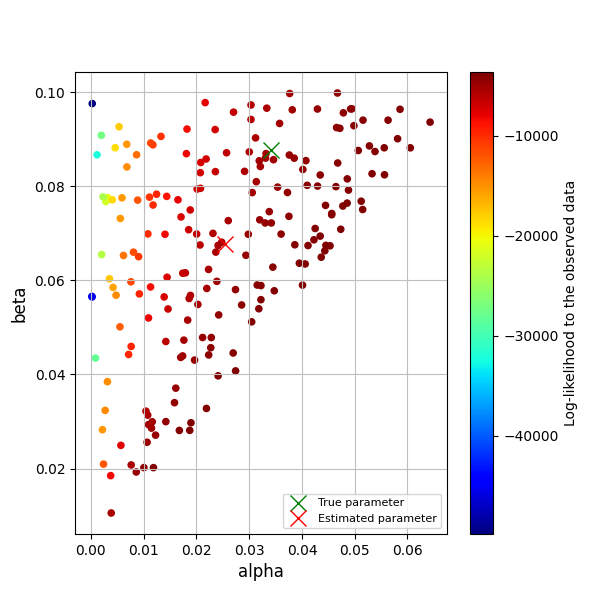
\includegraphics[width=\linewidth]{figures/sir510_rfsmc.png}
            \caption{Sampled particles using RF-SMC}
        \end{subfigure}
        \hfill
        \begin{subfigure}{0.4\textwidth}
            \centering
            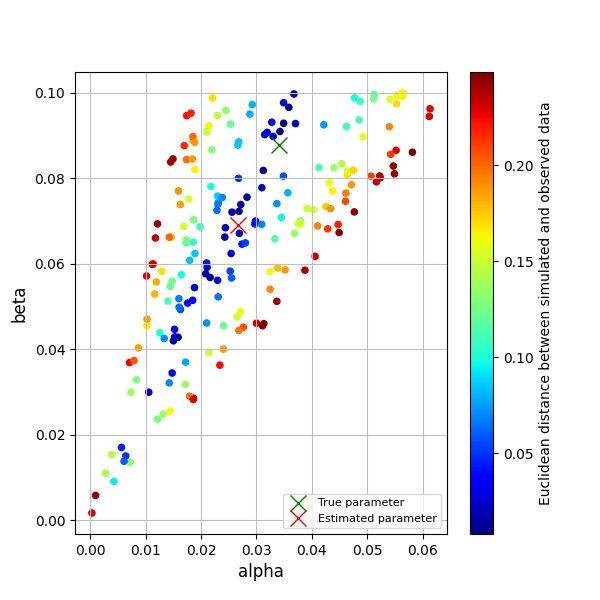
\includegraphics[width=\linewidth]{figures/sir510_abcsmc.png}
            \caption{Sampled particles using SMC-ABC-SMC}
        \end{subfigure}
        \caption{SIR(5,1,0) parameter synthesis results.}
    \end{figure}
\end{frame}

\begin{frame}
    \frametitle{SIR}
    \begin{table}[H]
        \centering
        \begin{tabular}{|l|l|l|}
            \hline
            Method                      & RF-SMC & SMC-ABC-SMC \\ \hline
            Total runtime (minutes)     & 19.567 & 231.60      \\ \hline
            \begin{tabular}[c]{@{}l@{}}Average perturbation\\ runtime (minutes)\end{tabular} & 1.03   & 11.838      \\ \hline
        \end{tabular}
        \caption{Physical runtime on SIR(5,1,0) model.}
    \end{table}
\end{frame}

\begin{frame}
    \frametitle{SIR}
    \begin{table}[H]
        \begin{tabular}{|l|l|l|}
            \hline
            Method                                           & RF-SMC               & SMC-ABC-SMC          \\ \hline
            Estimated parameter $\hat{\theta}$               & (0.014095, 0.066328) & (0.022552, 0.066416) \\ \hline
            True parameter $\theta$                          & (0.025490, 0.06930)  & (0.025490, 0.06930)  \\ \hline
            L2 distance $\Vert \theta, \hat{\theta} \Vert_2$ & 0.011776             & 0.004116             \\ \hline
            $P(\mathcal{M}_{\hat{\theta}}\models\Phi)$       & 0.363570             & 0.281154             \\ \hline
        \end{tabular}
        \caption{Parameter estimation results for SIR(10,1,0) model.}
    \end{table}
\end{frame}

\begin{frame}
    \frametitle{SIR}
    \begin{figure}[H]
        \centering
        \begin{subfigure}{0.48\textwidth}
            \centering
            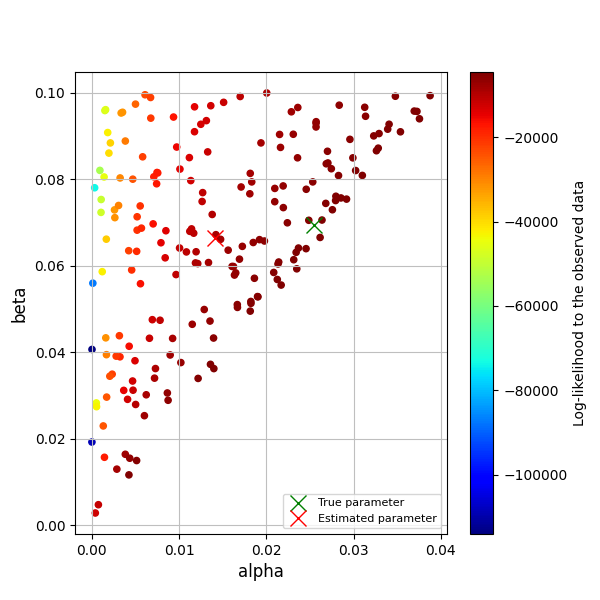
\includegraphics[width=\linewidth]{figures/sir1010_rfsmc.png}
            \caption{SIR(10,1,0), sampled particles using RF-SMC}
        \end{subfigure}
        \hfill
        \begin{subfigure}{0.48\textwidth}
            \centering
            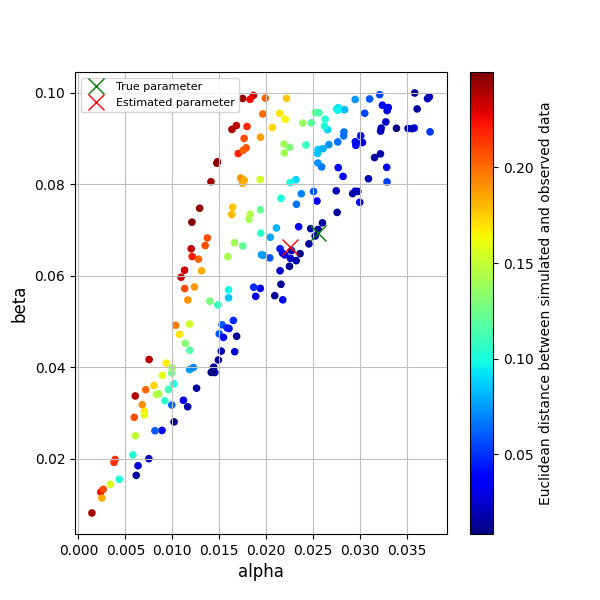
\includegraphics[width=\linewidth]{figures/sir1010_abcsmc.png}
            \caption{SIR(10,1,0), sampled particles using SMC-ABC-SMC}
        \end{subfigure}
        \caption{ parameter synthesis results.}
    \end{figure}
\end{frame}

\begin{frame}
    \frametitle{SIR}
    \begin{table}[H]
        \centering
        \begin{tabular}{|l|l|l|}
            \hline
            Method                      & RF-SMC  & SMC-ABC-SMC \\ \hline
            Total runtime (minutes)     & 165.033 & 567.683     \\ \hline
            \begin{tabular}[c]{@{}l@{}}Average perturbation\\ runtime (minutes)\end{tabular} & 8.685   & 26.962      \\ \hline
        \end{tabular}
        \caption{Physical runtime on SIR(10,1,0) model.}
    \end{table}
\end{frame}

\begin{frame}
    \frametitle{SIR}
    \begin{table}[H]
        \begin{tabular}{|l|l|l|}
            \hline
            Method                                           & RF-SMC               & SMC-ABC-SMC          \\ \hline
            Estimated parameter $\hat{\theta}$               & (0.012444, 0.065862) & (0.010022, 0.067230) \\ \hline
            True parameter $\theta$                          & (0.011499, 0.062111) & (0.011499, 0.062111) \\ \hline
            L2 distance $\Vert \theta, \hat{\theta} \Vert_2$ & 0.006545             & 0.005520             \\ \hline
            $P(\mathcal{M}_{\hat{\theta}}\models\Phi)$       & 0.366493             & 0.323579             \\ \hline
        \end{tabular}
        \caption{Parameter estimation results for SIR(15,1,0) model.}
    \end{table}
\end{frame}

\begin{frame}
    \frametitle{SIR}
    \begin{figure}[H]
        \centering
        \begin{subfigure}{0.48\textwidth}
            \centering
            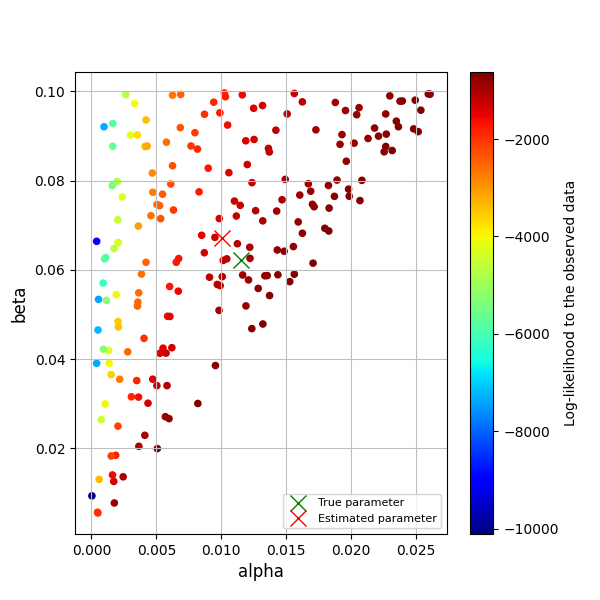
\includegraphics[width=\linewidth]{figures/sir1510_rfsmc.png}
            \caption{Sampled particles using RF-SMC}
        \end{subfigure}
        \hfill
        \begin{subfigure}{0.48\textwidth}
            \centering
            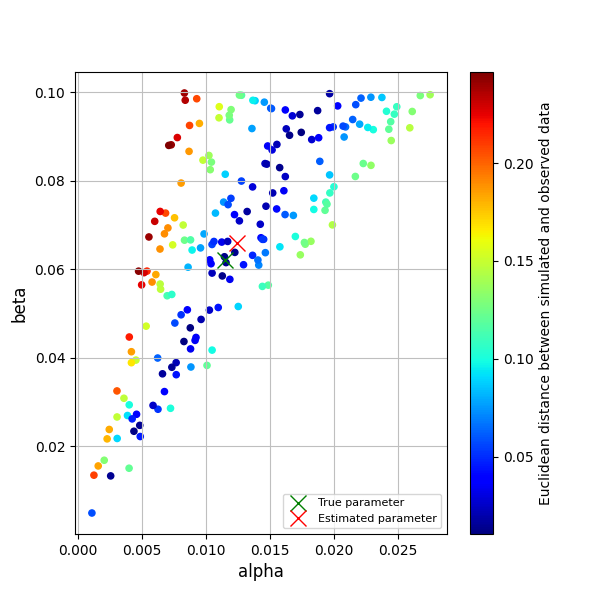
\includegraphics[width=\linewidth]{figures/sir1510_abcsmc.png}
            \caption{Sampled particles using SMC-ABC-SMC}
        \end{subfigure}
        \caption{SIR(15,1,0) parameter synthesis results.}
    \end{figure}
\end{frame}

\begin{frame}
    \frametitle{SIR}
    \begin{table}[H]
        \centering
        \begin{tabular}{|l|l|l|}
            \hline
            Method                      & RF-SMC & SMC-ABC-SMC \\ \hline
            Total runtime (minutes)     & 9657.0 & 776.9       \\ \hline
            \begin{tabular}[c]{@{}l@{}}Average perturbation\\ runtime (minutes)\end{tabular} & 50.814 & 37.945      \\ \hline
        \end{tabular}
        \caption{Physical runtime on SIR(15,1,0) model.}
    \end{table}
\end{frame}

\begin{frame}
    \frametitle{SIR result discussion}
    \begin{figure}[H]
        \centering
        \begin{subfigure}{0.48\textwidth}
            \centering
            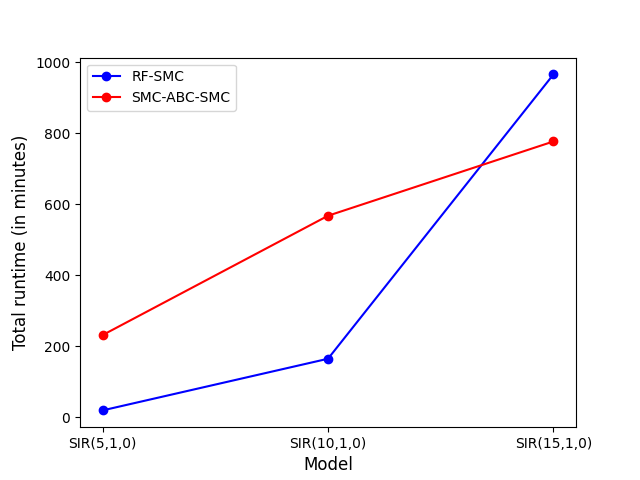
\includegraphics[width=\linewidth]{figures/sir_runtime_total.png}
            \caption{Total runtime}
        \end{subfigure}
        \hfill
        \begin{subfigure}{0.48\textwidth}
            \centering
            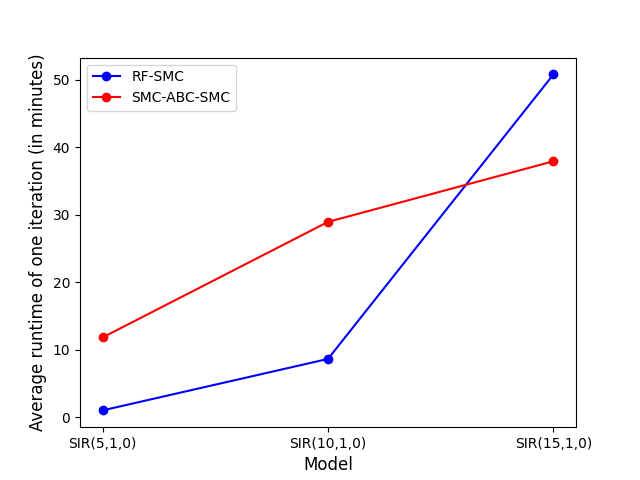
\includegraphics[width=\linewidth]{figures/sir_runtime_avg.png}
            \caption{Average perturbation runtime}
        \end{subfigure}
        \caption{Physical runtime on SIR models of different population sizes.}
    \end{figure}
    Result discussion:
    \begin{itemize}
        \item RF-SMC and SMC-ABC-SMC have comparable accuracy.
        \item From SIR(15,1,0), RF-SMC becomes much more expensive.
    \end{itemize}
\end{frame}


%%%%%%%%%%%%%%%%%%%%%%%%%%%%%%%%%%%%%%%%%%%%%%%%%%%%%%%%%%%%%%%%%%%%%%%%%%%%%%%%%%%%%%%%%%%%%%%%%%%%
\section{Conclusion and future work}
\begin{frame}
    \frametitle{Conclusion}
    \begin{itemize}
        \item The frameworks are tested against different case studies and show that they can
              deliver both a set of satisfying parameter values and an estimated parameter value
              close to the original value used to synthesize test data.
        \item As the number of states in a model grows, RF-SMC quickly becomes more expensive than
        SMC-ABC-SMC.
        \item We suggest that given an arbitrary parametric DTMC, simulation-based method
              SMC-ABC-SMC is preferable over the rational-function-based RF-SMC
    \end{itemize}
\end{frame}

\begin{frame}
    \frametitle{Future work}
    \begin{itemize}
        \item \textit{Statistical Model Checking}: using better bound for number of simulations
        \cite{molyneux2020abc}
        \item \textit{Bayesian Model Checking}: incorporating prior knowledge to perform Bayesian
              model checking to have closer estimation with less simulations Jha
              \cite{jha2009bayesian}, and Zuliani \cite{zuliani2013bayesian}.
        \item \textit{Sampling algorithms optimization}: number of particles, selection of
        perturbation function.
        \item \textit{Implementation improvement}: StormPy technically prohibits our implementation
              from being parallelized
              \footnote{\url{https://github.com/moves-rwth/stormpy/issues/36}}, so the only way to
              parallelize is to port to C++
    \end{itemize}
\end{frame}

%%%%%%%%%%%%%%%%%%%%%%%%%%%%%%%%%%%%%%%%%%%%%%%%%%%%%%%%%%%%%%%%%%%%%%%%%%%%%%%%%%%%%%%%%%%%%%%%%%%%
\begin{frame}[allowframebreaks]{References}
    \printbibliography
\end{frame}

\begin{frame}

    \begin{figure}[H]
        
\includegraphics[width=5cm]{figures/cat.jpeg}
        \caption{Thank you for your attention.}
    \end{figure}
\end{frame}

\end{document}